% latex models.tex ; dvips models.dvi ; ps2pdf models.ps
\documentclass{beamer}
\usepackage[latin1]{inputenc}
\usepackage{graphicx}
\usepackage{beamerthemesplit}
\usepackage{multicol,pgf,tikz}
\usetikzlibrary{shapes,arrows}
\usepackage{multimedia}
\usepackage{hyperref}
\usepackage{color}
\input{epsf}

\definecolor{durham}{cmyk}{0.5,0.8,0.,0.6}
%\setbeamercovered{transparent}
\mode<presentation>
{  \usetheme[height=7mm]{Rochester}
  \usecolortheme[named=durham]{structure}
  \useinnertheme[shadow]{rounded}
  \usefonttheme[onlymath]{serif}
  %\setbeamercovered{transparent}
  \setbeamertemplate{blocks}[rounded][shadow=true]
  \setbeamertemplate{navigation symbols}{} 
  %\setbeamertemplate{footline}{\hspace{12cm} \insertframenumber/\inserttotalframenumber
  \setbeamertemplate{footline}{V. Gonzalez-Perez \hspace{10.2cm} \insertframenumber/\inserttotalframenumber }
}

%%%%%%%%%%%%%%%%
\newcommand{\lcdm}{$\rm{\Lambda CDM}$}
\newcommand{\gl}{\textsc{galform}}
\newcommand{\eg}{\textsc{eagle}}
\newcommand{\egdm}{\textsc{eagleDMO}}
\newcommand{\lgl}{\textsc{l-galaxies}}
\newcommand{\subf}{\textsc{subfind}}
\newcommand{\msun}{{\rm M}_{\odot}}
\newcommand{\mb}{M_{\rm Break}}
\newcommand{\mth}{{\rm M}_{200}^{\rm crit}}
\newcommand{\mtry}{\todo[\textcolor{blue}{Upd.}]}
\newcommand{\stry}{\todo[\textcolor{blue}{From Shaun: Upd.}]}
\newcommand{\ptry}{\todo[\textcolor{blue}{From Peter: Upd.}]}
\newcommand{\nm}{$\langle N \rangle_{M}$}
%%%%%%%%%%%%%%%%

\title{Comprehensive models of galaxy formation and evolution}
\author{{\bf Violeta Gonzalez-Perez}}
\institute{@violegp\\
}
\date{}


\begin{document}
\frame{\titlepage 
\vspace{-0.5cm}
\begin{center}
\includegraphics[height=0.25\textheight]{/home/violeta/charlas/fig/logos/icg-logo.ps}
\end{center}
}



%%_____Flow charts_____________________________________
\tikzstyle{decision} = [diamond, draw=green!50!black!50,fill=green!50!black!50, text centered, text width=3.8em]
\tikzstyle{up} = [rectangle, draw, very thick,
draw=blue!50!black!50,level distance=4cm,
    text width=15em, text centered, rounded corners, minimum height=8em]
\tikzstyle{down} = [rectangle, draw, very thick,
draw=red!50!black!50,level distance=4cm,
    text width=5em, text centered, rounded corners, minimum height=3em]
\tikzstyle{up1} = [rectangle, draw, very thick,
draw=blue!50!black!50,level distance=4cm,
    text width=5em, text centered, rounded corners, minimum height=5em]
\tikzstyle{down1} = [rectangle, draw, very thick,
draw=red!50!black!50,level distance=4cm,
    text width=5em, text centered, rounded corners, minimum height=5em]
\tikzstyle{up2} = [rectangle, draw, very thick,
draw=blue!50!black!50,level distance=4cm,
    text width=10em, text centered, rounded corners, minimum height=8em]
\tikzstyle{sed} = [rectangle, draw, very thick,
draw=green!50!black!50,level distance=4cm,
    text width=5em, text centered, rounded corners, minimum height=7em]
\tikzstyle{thing} = [rectangle, draw, very thick,
draw=red!50!black!50,level distance=4cm,
    text width=4em, text centered, rounded corners, minimum height=2em]
\tikzstyle{line} = [draw, -latex]
\tikzstyle{cloud} = [draw, ellipse,fill=black]   
\tikzstyle{newm} = [draw=green!50!black!50, ellipse,fill=green!50!black!50,text width=4em,text centered]   
\tikzstyle{prop} = [circle,fill=red, level distance=1cm,text width=5em,text centered]   
\tikzstyle{empty} = [minimum height=2em]   


%%_____Introduction______________________________________

\begin{frame}{The Millennium simulation}
\begin{center}
\movie[autostart]{\includegraphics[height=0.7\textheight]{/home/violeta/charlas/fig/intro/millennium.ps}}{millennium.avi}
\end{center}
\end{frame}

\begin{frame}{An excercise}
\begin{itemize}
\item Simulation: \url{http://virgodb.cosma.dur.ac.uk:8080/Millennium/}

Millimillenium box size = $62.5$ Mpc$h^{-1}$ \\
Mass of each dark matter particle = $8.6\cdot 10^8$M$_{\odot}h^{-1}$
\item Data: \url{http://www.astro.ljmu.ac.uk/~ikb} \\ \url{/research/gama-gsmf-paper.html}
\end{itemize}
\end{frame}


\begin{frame}{Query for getting the dark matter mass function}
\texttt{select .1*(.5+floor((log10(np*0.86)+9.)/.1)) as mass, \\
       log10(count(*)/power(62.5,3.)/.1) as phi \\
from millimil..MPAHalo \\
where snapnum=63 \\
group by .1*(.5+floor((log10(np*0.86)+9.)/.1)) \\
order by mass   
}
\end{frame}

\begin{frame}{The mass function}
Plotting directly the output from the query: mass vs phi
\begin{center}
\includegraphics[height=0.7\textheight]{/home/violeta/teaching/lecture2016.port/db_mf/mf.ps}
\end{center}
\end{frame}


\begin{frame}{The galaxy stellar mass function}
Plotting the galaxy stellar mass function from observations (Baldry et al. 2008) together with the Schechter function derived by Panter et al. 2007:
\begin{center}
\includegraphics[height=0.7\textheight]{/home/violeta/teaching/lecture2016.port/db_mf/obs_gsmf.ps}
\end{center}
\end{frame}


\begin{frame}{The galaxy stellar mass function }
Let's compare the observed the galaxy stellar mass function with that derived from the dark matter mass function (mass and phi from the query) by multiplying it by the baryonic fraction ($M_{*}=M_{\rm halo}\cdot f_b$)
\begin{center}
\includegraphics[height=0.7\textheight]{/home/violeta/teaching/lecture2016.port/db_mf/mhfb.ps}
\end{center}
\end{frame}


\begin{frame}{The galaxy stellar mass function }
Let's normalized the galaxy stellar mass function around the knee of the observed one ($M_{*}=N\cdot M_{\rm halo}\cdot f_b$):
\begin{center}
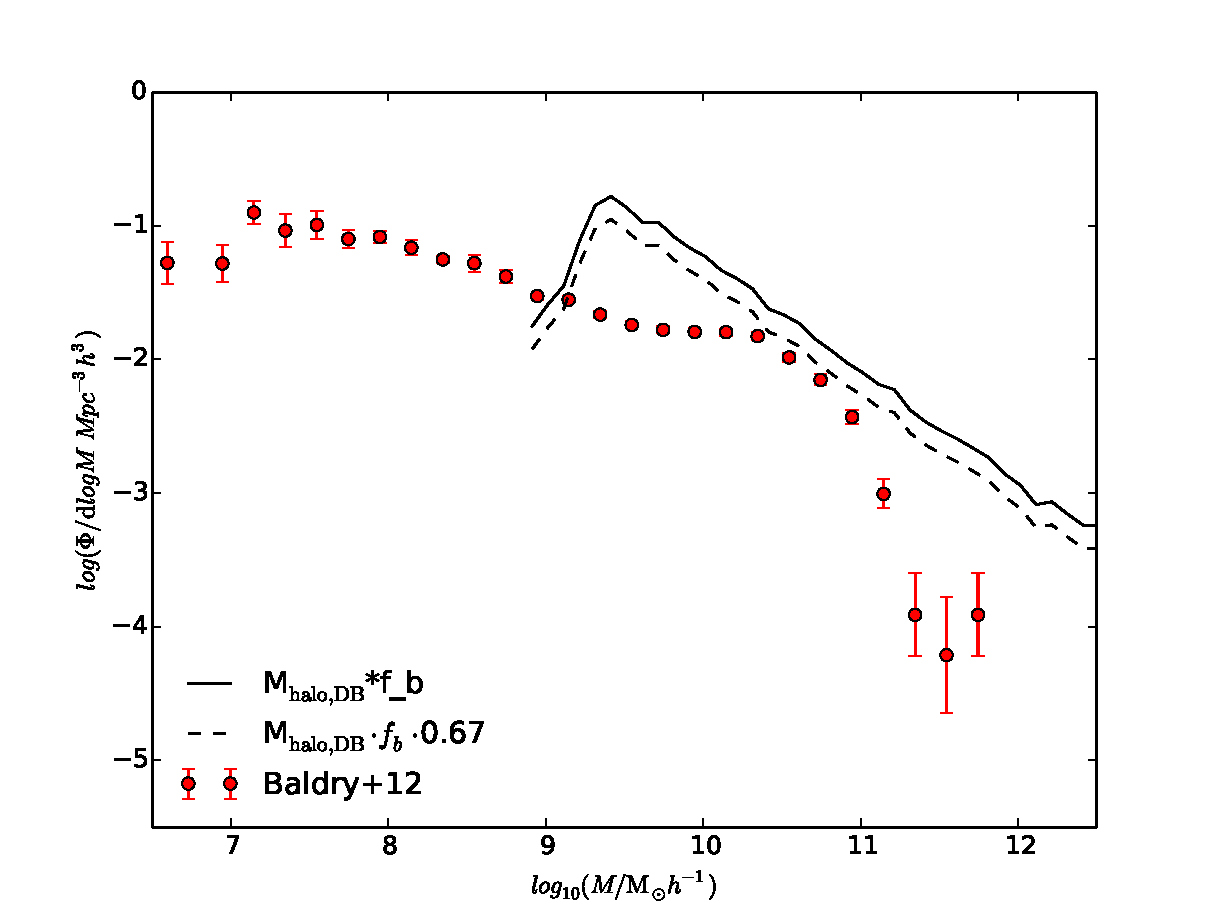
\includegraphics[height=0.7\textheight]{/home/violeta/teaching/lecture2016.port/db_mf/mhfbnorm.ps}
\end{center}
The shapes are still different! We need a better model to connect the luminose matter to the dark one.
\end{frame}


\begin{frame}{Making galaxies in the computer {\small with a semi-analytical model}}
\begin{tikzpicture}[node distance = 2cm, auto]
    \node [cloud] (cosmo) {\textcolor{white}{$\Lambda$CDM   Cosmology}}; 
    \node [cloud, below of=cosmo, yshift=1cm] (dm) {\textcolor{white}{DM Merger trees}}; 
    \node [decision, below of=dm] (cool) {\textcolor{white}{Efficient cooling?}}; 
   \node [empty, below of=cool, xshift=-0.4cm, yshift=0.4cm] (yescool) {\textcolor{green!50!black!50}{Yes}};
   \node [empty, left of=cool, xshift=0.4cm, yshift=0.2cm] (nocool) {\textcolor{green!50!black!50}{No}};
    \node [thing, left of=cool, xshift=-1cm] (dh) {Dark Halo}; 
    \node [decision, below of=cool, yshift=-1cm] (jm) {\textcolor{white}{Large j?}}; 
   \node [empty, right of=jm, yshift=1cm, xshift=-1.2cm, rotate=40 ] (yesj) {\textcolor{green!50!black!50}{Yes}};
   \node [empty, right of=jm, yshift=-1cm, xshift=-1.2cm, rotate=-40] (noj) {\textcolor{green!50!black!50}{No}};
    \node [thing, right of=jm, yshift=1.5cm] (disc) {Disc}; 
    \node [thing, right of=jm, yshift=-1.5cm] (bulge) {Bulge}; 
    \node [decision, right of=jm,xshift=1.5cm] (merge) {\small \textcolor{white}{Merger? Disc instability?}}; 
    % Draw edges
    \path [line, thick] (cosmo) -> (dm); \path [line, thick] (dm) -> (cool);
    \path [line, thick] (cool) -> (dh); \path [line, thick] (dh) -> (dm);
    \path [line, thick] (cool) -> (jm); \path [line, thick] (jm) -> (disc);
    \path [line, thick] (disc) -> (merge); \path [line, thick] (jm) -> (bulge);
    \path [line, thick] (merge) -> (bulge); 
\end{tikzpicture}
\end{frame}

\begin{frame}{The model baryonic component in a halo}
\includegraphics[height=1\textheight]{/home/violeta/charlas/fig/intro/lagos_chart.ps}
\end{frame}
%

\begin{frame}{The semi-analytical approach}
\begin{center}
\movie[autostart]{\includegraphics[height=0.7\textheight]{/home/violeta/charlas/fig/intro/gal_dm.eps}}{movie}
\end{center}
\end{frame}


\begin{frame}{Query for getting the stellar mass function}
The following query gets the galaxy stellar mass function from the De Lucia et al. 2006 model, which is a comprehensive model of galaxy formation and evolution:


\texttt{select .1*(.5+floor((log10(stellarMass)+10.)/.1)) as mass, \\
		        log10(count(*)/power(62.5,3.)/.1) as phi \\
		   from millimil..DeLucia2006a \\
	where snapnum = 63 and stellarMass > 0 \\
	group by .1*(.5+floor((log10(stellarMass)+10.)/.1)) \\
	order by mass 
}
\end{frame}


\begin{frame}{The galaxy stellar mass function}
Plotting the result of the previous query, together with the other results:
\begin{center}
\includegraphics[height=0.7\textheight]{/home/violeta/teaching/lecture2016.port/db_mf/sam.ps}
\end{center}
\end{frame}


%\begin{frame}{The \eg~ simulation}
%\movie[autostart]{\includegraphics[height=0.9\textheight]{/home/violeta/charlas/fig/eagle/eagle_movie.eps}}{movie2}
%\end{frame}
%
%
%\begin{frame}{A closer look to the Star Formation}
%\tikzstyle{decision} = [diamond, draw=green!50!black!50,fill=green!50!black!50, text centered, text width=3.8em]
%\tikzstyle{up} = [rectangle, draw, very thick,
%draw=blue!50!black!50,level distance=4cm,
%    text width=15em, text centered, rounded corners, minimum height=8em]
%\tikzstyle{down} = [rectangle, draw, very thick,
%draw=red!50!black!50,level distance=4cm,
%    text width=5em, text centered, rounded corners, minimum height=3em]
%\tikzstyle{up1} = [rectangle, draw, very thick,
%draw=blue!50!black!50,level distance=4cm,
%    text width=5em, text centered, rounded corners, minimum height=5em]
%\tikzstyle{down1} = [rectangle, draw, very thick,
%draw=red!50!black!50,level distance=4cm,
%    text width=5em, text centered, rounded corners, minimum height=5em]
%\tikzstyle{sed} = [rectangle, draw, very thick,
%draw=green!50!black!50,level distance=4cm,
%    text width=5em, text centered, rounded corners, minimum height=7em]
%\tikzstyle{line} = [draw, -latex]
%\tikzstyle{cloud} = [draw, ellipse,fill=black]   
%\tikzstyle{newm} = [draw=green!50!black!50, ellipse,fill=green!50!black!50,text width=4em,text centered]   
%\tikzstyle{prop} = [circle,fill=red, level distance=1cm,text width=5em,text centered]   
%\tikzstyle{empty} = [minimum height=2em]   
%
%\begin{tikzpicture}[node distance = 2cm, auto]
%    % Place nodes
%    \node [empty,xshift=-2cm] (galform) {\includegraphics[height=0.15\textheight]{/home/violeta/charlas/fig/galform.eps}};
%   \node [up, right of=galform,xshift=3.5cm,yshift=1cm] (disk) {\small \textcolor{durham}{ Using analytical equations, containing free parameters, {\sc galform} calculates the physical processes affecting the evolution of galaxies:
%\hspace{-0.5cm}{\begin{itemize}
%\item Gas cooling $\Rightarrow$ Disk formation 
%\item Galaxy mergers $\Rightarrow$ Spheroids
%\item SF{\color{red}$^*$} \& Feedback \\ \hspace{1cm}{\color{red} from both SNe \& AGN}
%\item Chemical Evolution
%\item Stellar population \& Extinction
%\end{itemize}}
%}};
%    \node [cloud, above of=galform] (dm) {\textcolor{white}{DM Merger trees}}; 
%    \node [cloud, above of=dm,yshift=-1cm] (cosmo) {\textcolor{white}{$\Lambda$CDM   Cosmology}}; 
%%%
%%%
%    % Draw edges
%    \path [line, thick] (cosmo) -> (dm);
%    \path [line, thick] (dm) -> (galform);
%%
%\end{tikzpicture}
%{\color{red}$^*$} New improved treatment of SF in disks ({\color{durham}Lagos et al. 2011}) based on the empirical law from Blitz \& Rosolowsky (2006), following explicitly the He, HI \& H$_2$:
%\begin{equation*}
%\Sigma _{SFR}= \frac{1}{\tau _{mol.\, gas}}\times \frac{\Sigma _{mol.\, gas}}{\Sigma _{total\, gas}}(\rm{P_{hydrostatic}\, of\, the\, disk})\times \Sigma _{cold\, gas}
%\end{equation*} 
%\end{frame}

%-----------------------------------------------
\end{document}
